\documentclass[a4paper,11pt]{article}
\usepackage{a4wide}
\usepackage{fullpage}
\usepackage[utf8x]{inputenc}

\usepackage[light,math]{anttor}
\usepackage[T1]{fontenc}

%\usepackage[slovene]{babel}
%\selectlanguage{slovene}
\usepackage[toc,page]{appendix}
\usepackage[pdftex]{graphicx} 

\usepackage{lmodern}
\usepackage{amsmath}
\usepackage{amssymb}
\usepackage{amsthm}
\usepackage{amsfonts}
\usepackage{mathtools}
\usepackage{enumitem}
\usepackage{amsfonts}
\usepackage{amsmath}
\usepackage{setspace}
\usepackage{color}
\definecolor{light-gray}{gray}{0.95}
\usepackage{listings} 
\usepackage{hyperref}
\renewcommand{\baselinestretch}{1.2} 
\renewcommand{\appendixpagename}{Priloge}


\title{Analysis of electromyogram of uterus (EHG) \\
using sample entropy}
\author{Sara Bizjak}
\date{\today}

\begin{document}

\maketitle

\section{Abstract}

\ \ 
This paper represents results of EHG analysis using non-linear processing techique \textit{sample theory}, tested on \cite{bib:fisio}. 
\section{Introduction}

\ \
Uterine electromyogram (EMG), also termed electrohysterogram (EHG), represents electrical activity of uterus.
The EHG signals contain also intervals with increased electrical activity of the uterus. 
The increased electrical activity is visible in the EHG signals as short bursts with higher signal amplitude. 
These intervals usually coincide with contractions -- but not all intervals with increased electrical activity of the uterus are a result of contractions. 
The frequency contents of the EHG signal changes during contractions, 
but the studies have also shown, that the frequency contents of the EHG signals as well as frequency contents of individual contractions within a signal, changes as the labour approaches.
\\
Using the EHG, it is possible to automatically detect uterine electical activity during both gestation and active labor. Therefore, with the help of EHG, the prediction of the premature labor (pregnancy duration less than $37$ weeks) can be done, 
since using risk factors, such as diabetes, hypertension, abnormalities of the uterus,... is far from certain.
Successful prediction of premature labor would confirm the use of oxytocin antagonist sooner in the process of pre-term delivery. 
\\
\\
The EHG analysis consists of records of term delivers (duration $>= 37$ weeks) and prematurely delivers (pregnancy duration $< 37$ weeks). 
Some records were obtained before the $26^{th}$ week and some during or after the $26^{th}$ week of gestation:
\begin{itemize}
    \item PE : pre-term labour, recorded before $26^{th}$ week,
    \item PL : pre-term labour, recorded during or after $26^{th}$ week
    \item TE : term labour, recorded before $26^{th}$ week
    \item TL : term labour, recorded during or after $26^{th}$ week
\end{itemize}

\section{Methodology}

\subsection{Terms}
\ \
The Butterworth filter is a type of signal processing filter designed to have as flat a frequency response as possible in the passband and is computationally non intensive.
Filter can be low-pass, high-pass or band-pass. For calculations presented in this paper, band-pass filter is used.
\\
The sample entropy is a measure of regularity of finite length time series and estimates the extent to which the data did not arise from a random process.
Less predictable time series exhibit a higher sample entropy. 
Given a time series $u[n]$ of length $N$ (from where we take the patterns as $a_j[i] = u[i + j], i = 0, \ldots, m - 1$ and  $j = 0, \ldots, N - m$) and petterns $a_j[0, \ldots, m - 1]$ of length $m$, where $m < N$ we count the pattern matches (where the difference is at most as determined pattern match margin $r$).
The number of pattern matches $c_m$ -- within a margin of $r$ -- is constructed for each $m$.
The sample entropy is then defined as:
\begin{displaymath}
    \text{sampleEntropy}_{m, r}(x) = \left\{ \begin{array}{ll}
     - \text{log} \left( \frac{c_m}{c_{m-1}} \right) & \ , \ c_m \neq 0 \ \text{and} \ c_{m-1} \neq 0 \\
     - \text{log} \left( \frac{N - m}{N - m - 1} \right) & \ , \ c_m = 0 \ \text{or} \ c_{m-1} = 0 \\
    \end{array}  \right.
\end{displaymath}

\subsection{Usage}
\ \ 
Evaluation of sample entropy to separate groups of records according to delivery time is made on 0.3-4 Hz band-pass preprocessing filtered records.


\section{Results}
\ \ 
On the pictures below are presented (shorted) clips of original and filtered records from all four groups (PE, PL, TE, TL) on $3^{rd}$ signal.

\begin{figure}[ht!]
    \begin{minipage}{0.5\textwidth}
        \centering
        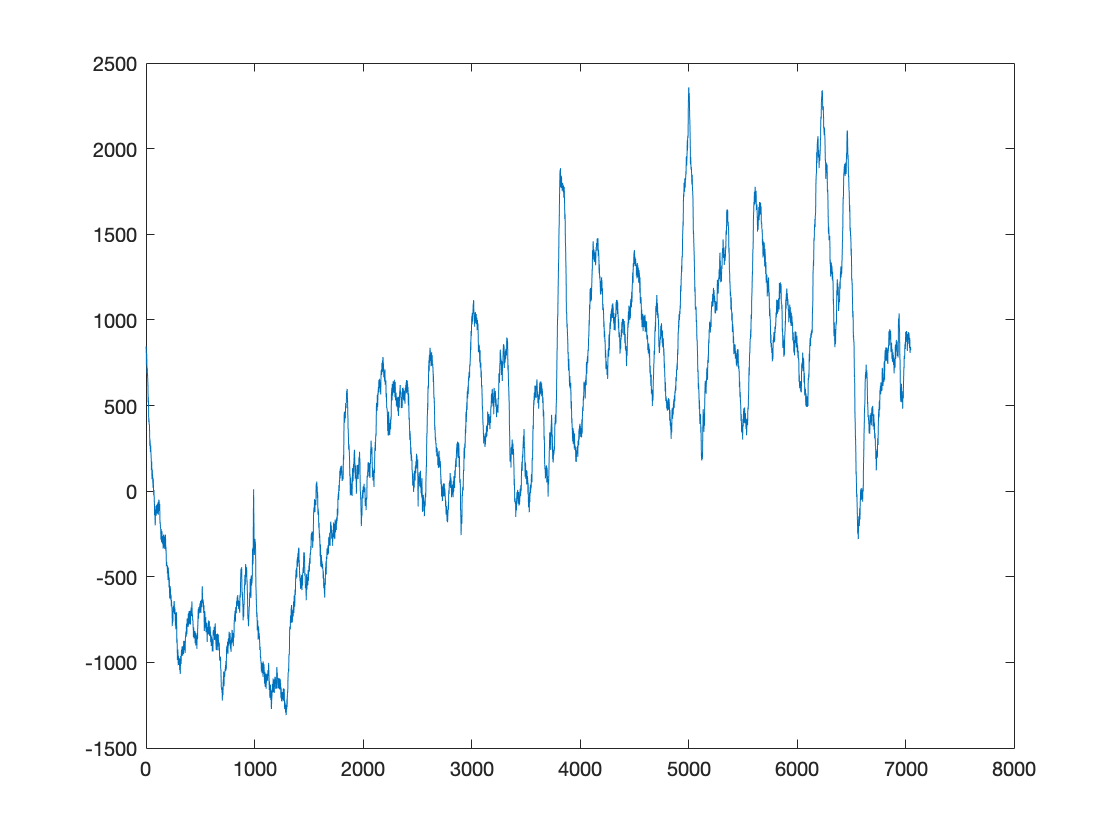
\includegraphics[width=70mm]{PE_sig3.png}
        \caption{Unfiltered PE record of $3^{rd}$ signal.}
    \end{minipage}\hfill
    \begin{minipage}{0.5\textwidth}
        \centering
        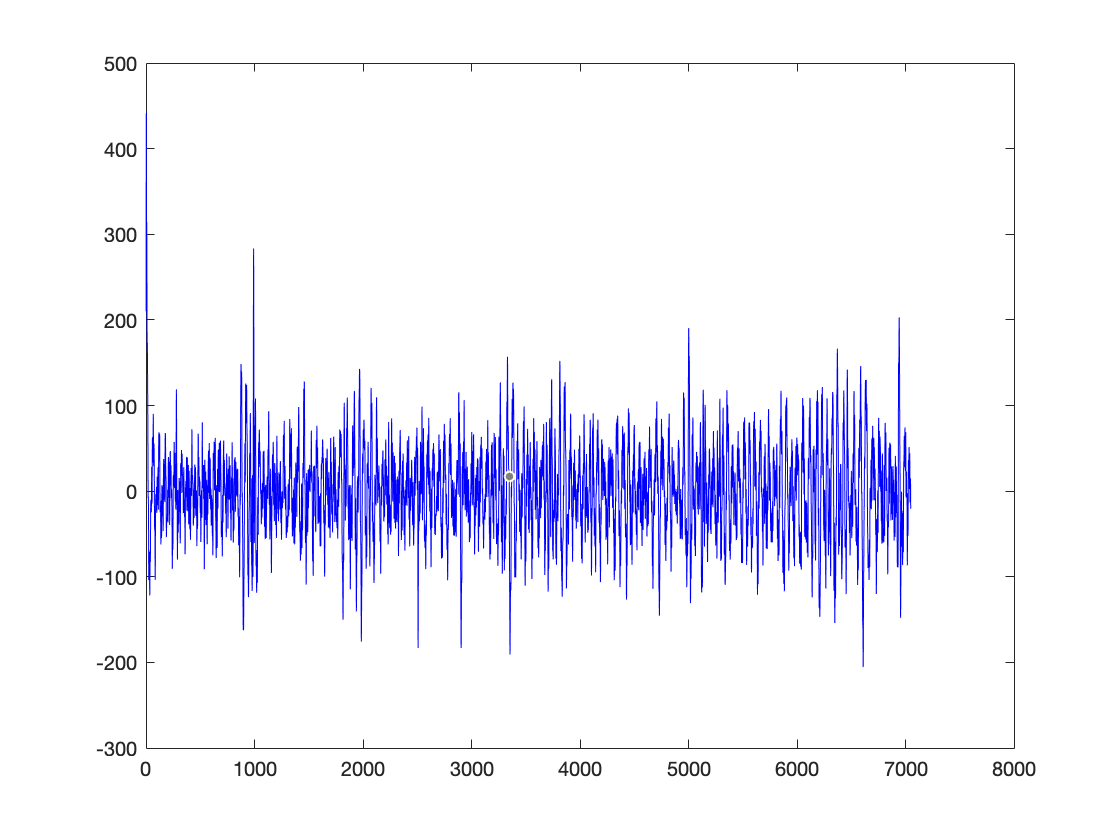
\includegraphics[width=70mm]{PE_sig3_filtered.png}
        \caption{Filtered PE record of $3^{rd}$ signal.}
    \end{minipage}\hfill
\end{figure}
\newpage
\begin{figure}[ht!]
    \begin{minipage}{0.5\textwidth}
        \centering
        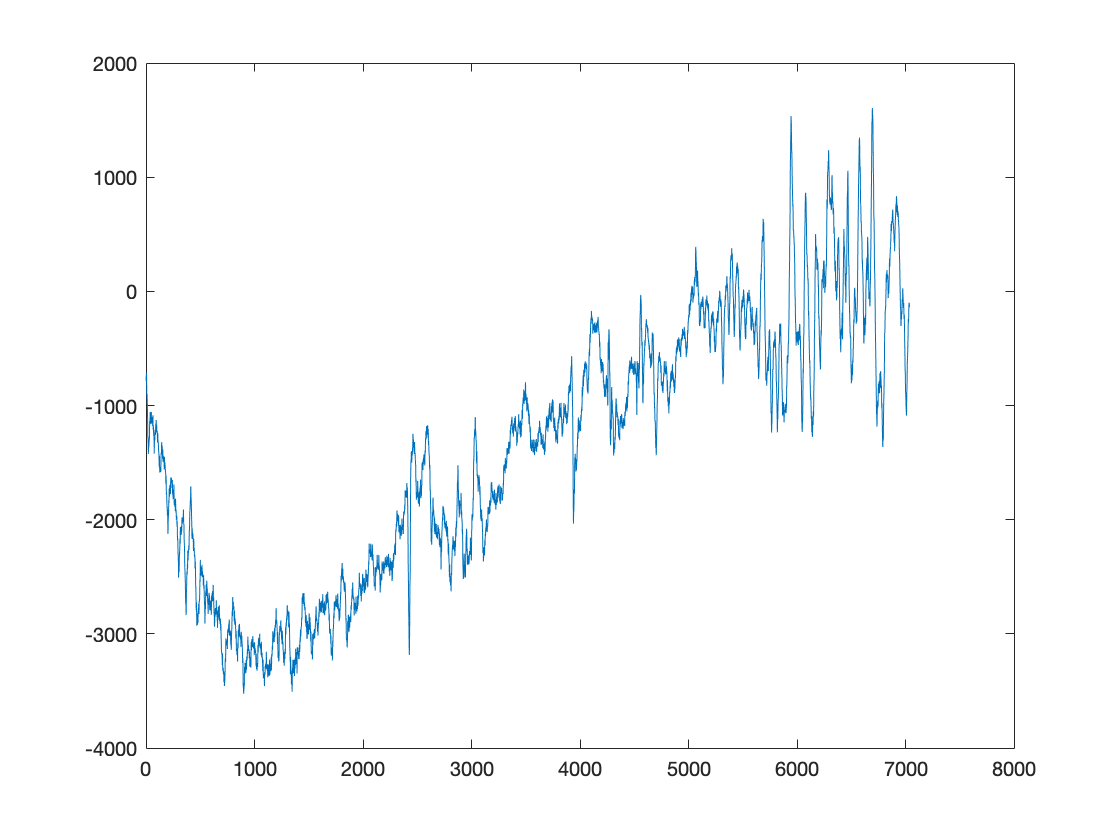
\includegraphics[width=70mm]{PL_sig3.png}
        \caption{Unfiltered PL record of $3^{rd}$ signal.}
    \end{minipage}\hfill
    \begin{minipage}{0.5\textwidth}
        \centering
        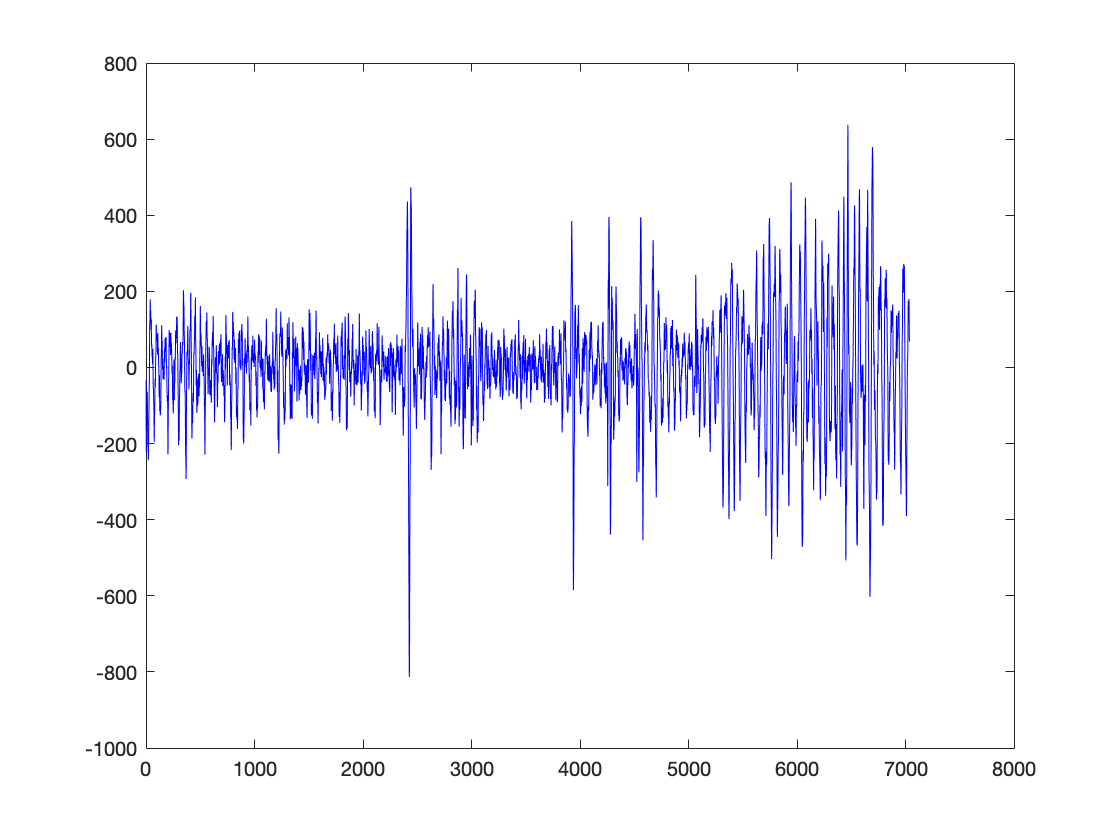
\includegraphics[width=70mm]{PL_sig3_filtered.png}
        \caption{Filtered PL record of $3^{rd}$ signal.}
    \end{minipage}\hfill
\end{figure}

\begin{figure}[ht!]
    \begin{minipage}{0.5\textwidth}
        \centering
        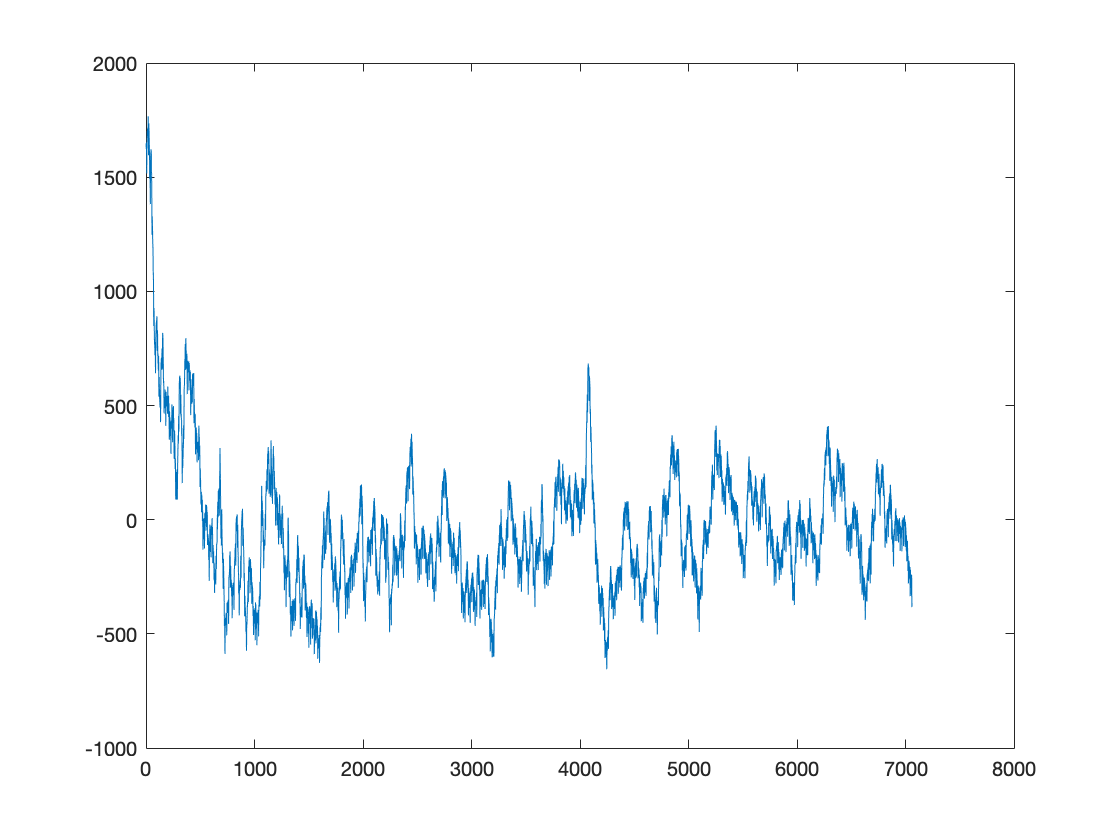
\includegraphics[width=70mm]{TE_sig3.png}
        \caption{Unfiltered TE record of $3^{rd}$ signal.}
    \end{minipage}\hfill
    \begin{minipage}{0.5\textwidth}
        \centering
        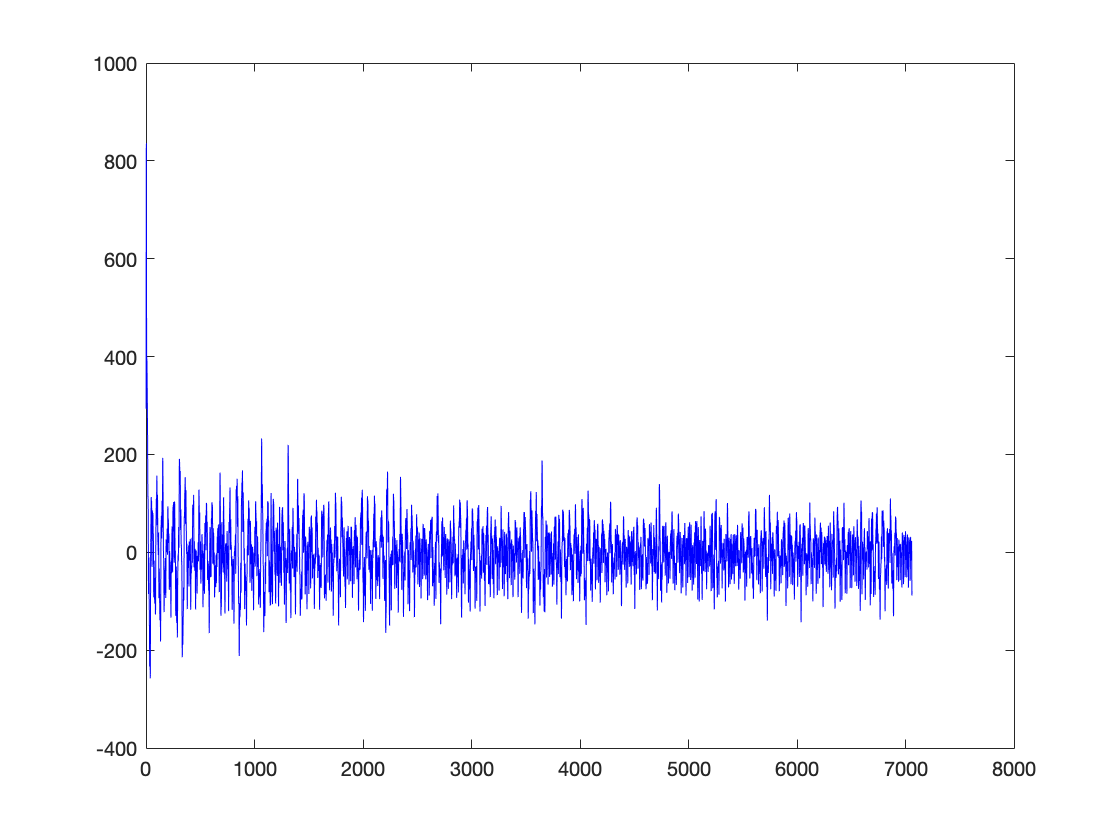
\includegraphics[width=70mm]{TE_sig3_filtered.png}
        \caption{Filtered TE record of $3^{rd}$ signal.}
    \end{minipage}\hfill
\end{figure}

\begin{figure}[ht!]
    \begin{minipage}{0.5\textwidth}
        \centering
        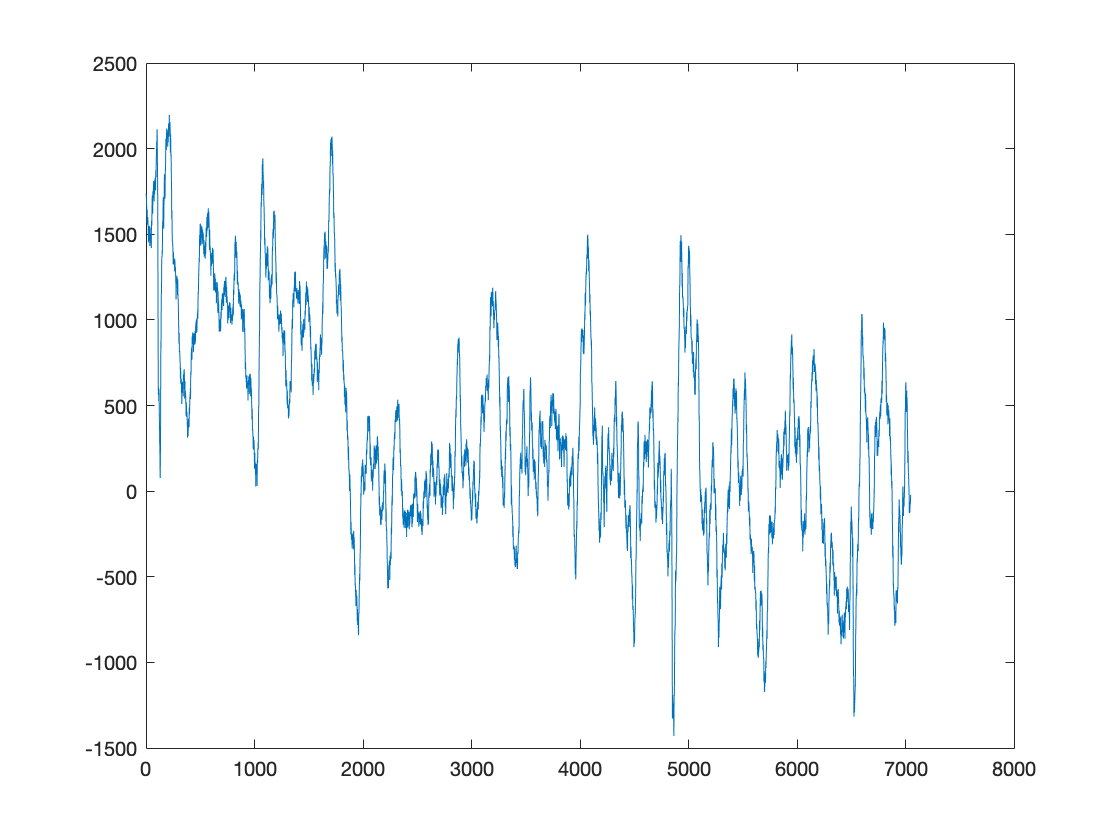
\includegraphics[width=70mm]{TL_sig3.png}
        \caption{Unfiltered TL record of $3^{rd}$ signal.}
    \end{minipage}\hfill
    \begin{minipage}{0.5\textwidth}
        \centering
        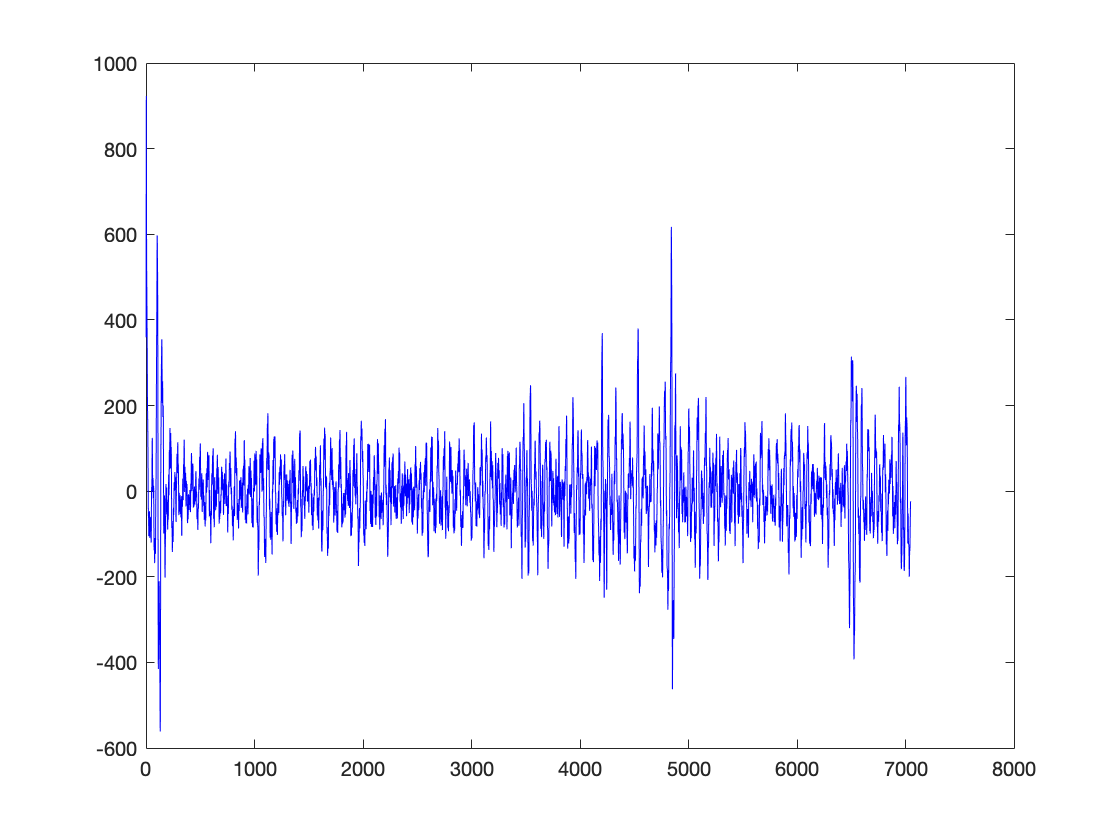
\includegraphics[width=70mm]{TL_sig3_filtered.png}
        \caption{Filtered TL record of $3^{rd}$ signal.}
    \end{minipage}\hfill
\end{figure}
\newpage
\noindent
In the pictures below are presented all filtration stages (on TL record) and two spectrograms (one of TL and one of PL record).
\begin{figure}[ht!]
    \centering
    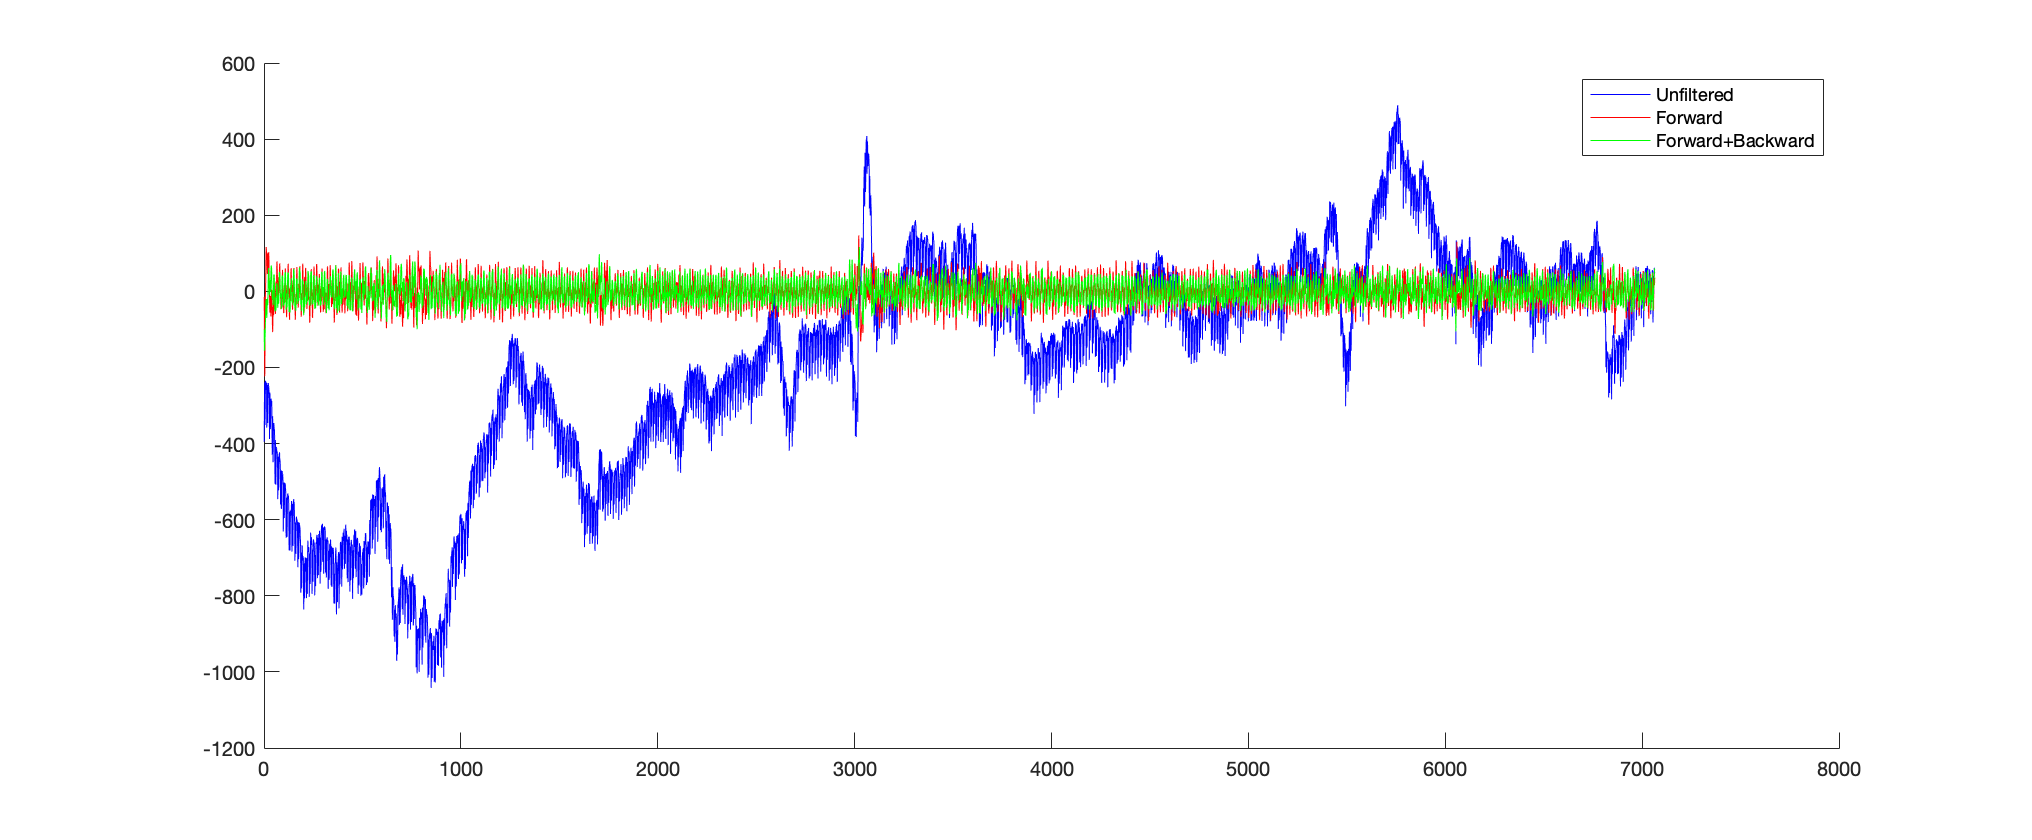
\includegraphics[width=150mm]{TL_butter.png}
    \caption{Visualisation of the filtration process with Butter filter (on TL record).}
\end{figure}

%\begin{figure}[ht!]
%    \centering
%    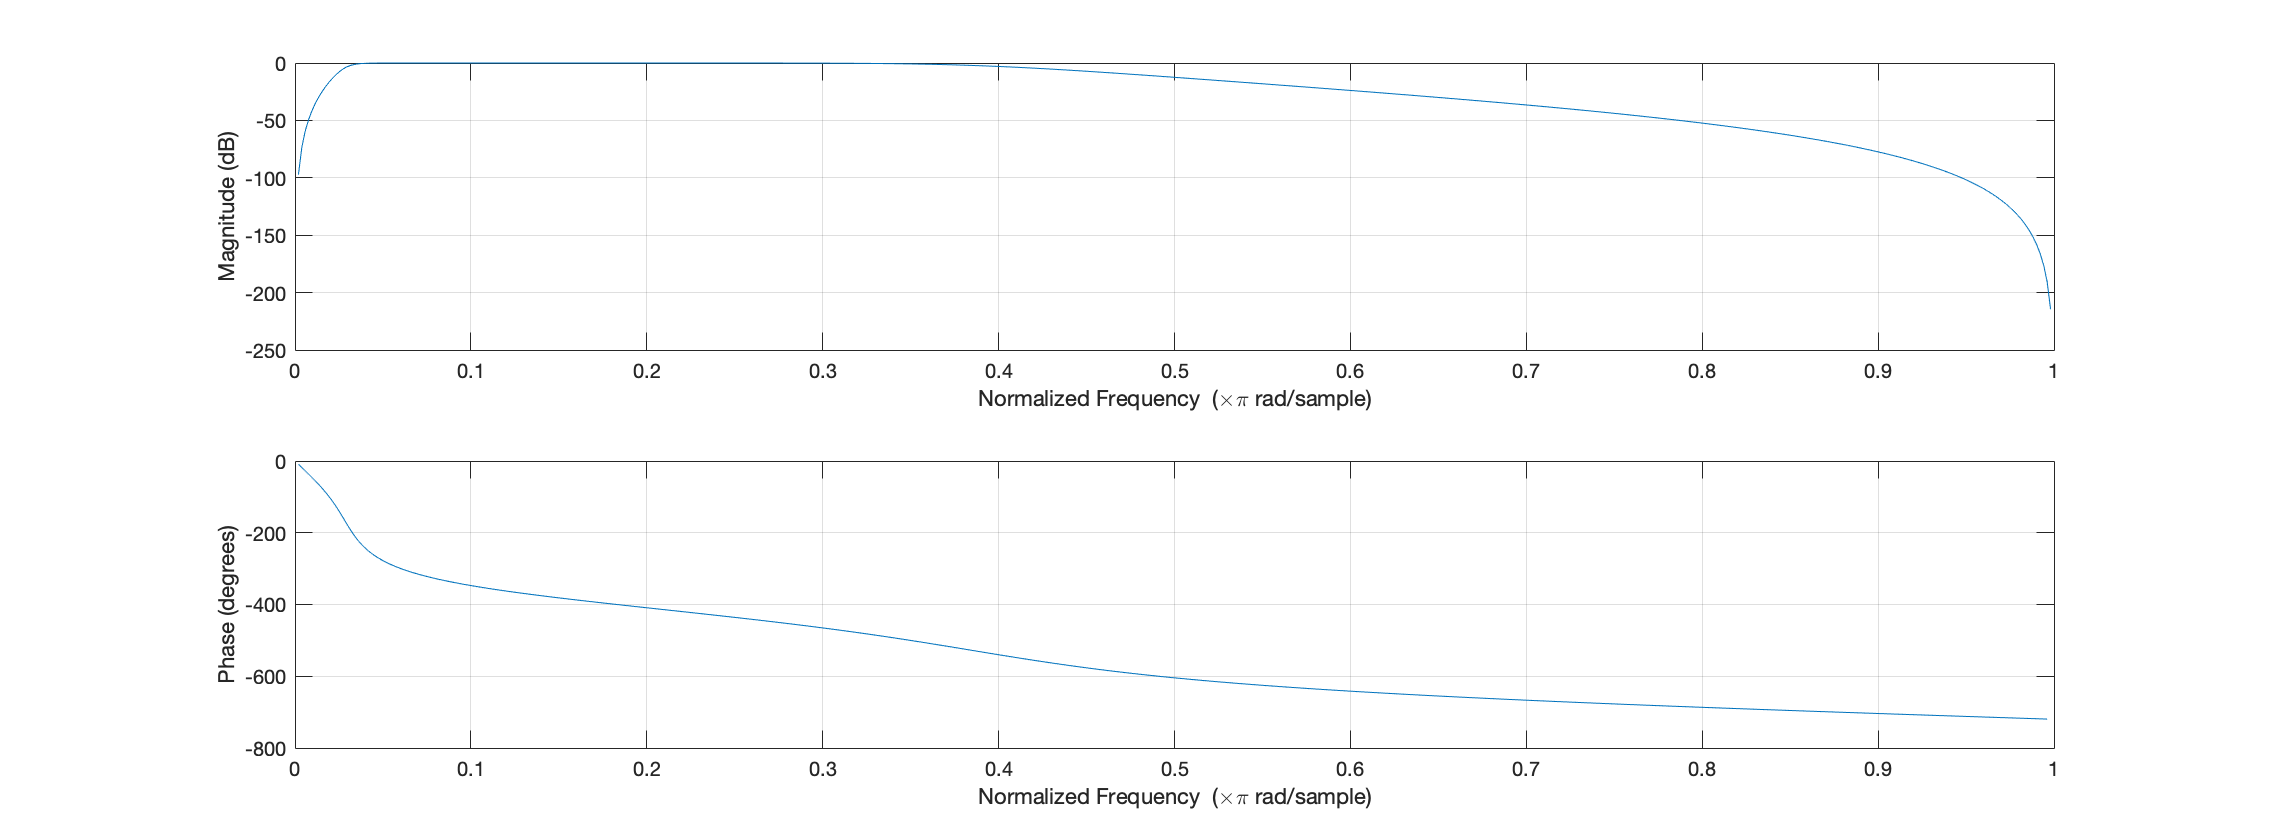
\includegraphics[width=130mm]{TL_freqz.png}
%    \caption{Frequency (magnitude and phase) response of the designed Butterworth filter (on TL record).}
%\end{figure}

\begin{figure}[ht!]
    \begin{minipage}{0.5\textwidth}
        \centering
        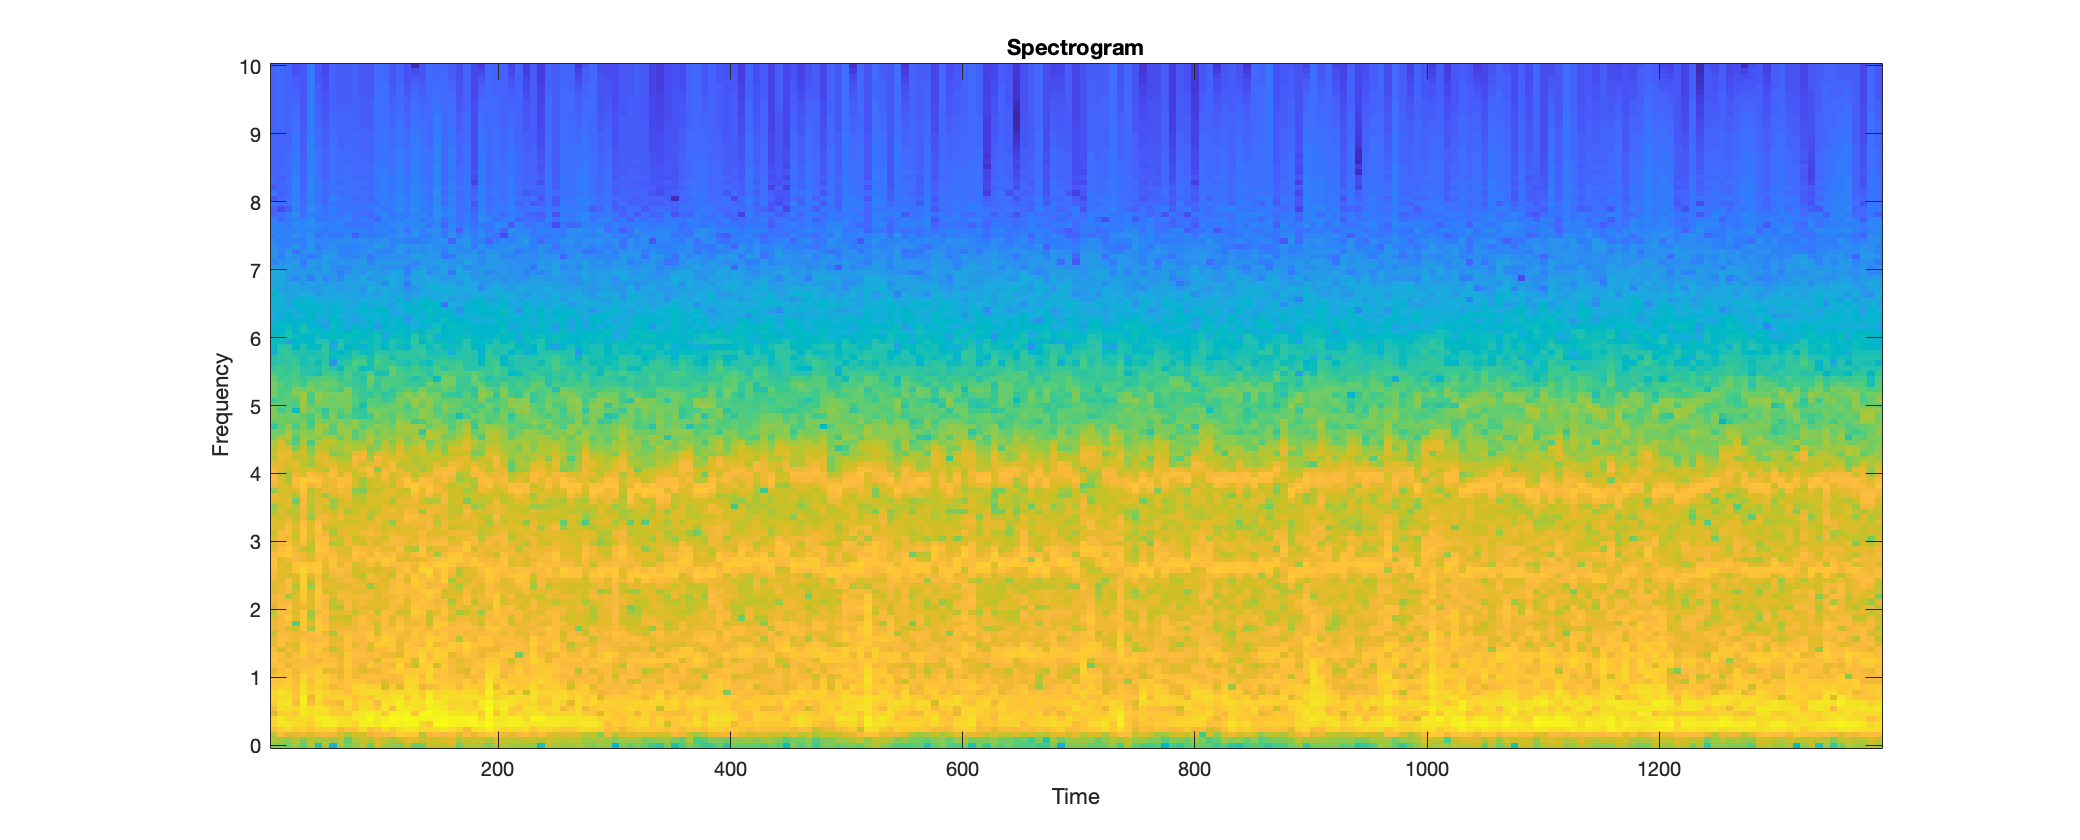
\includegraphics[width=85mm]{PL_sig3_spectrogram.png}
        \caption{Spectrogram of PL record.}
    \end{minipage}\hfill
    \begin{minipage}{0.5\textwidth}
        \centering
        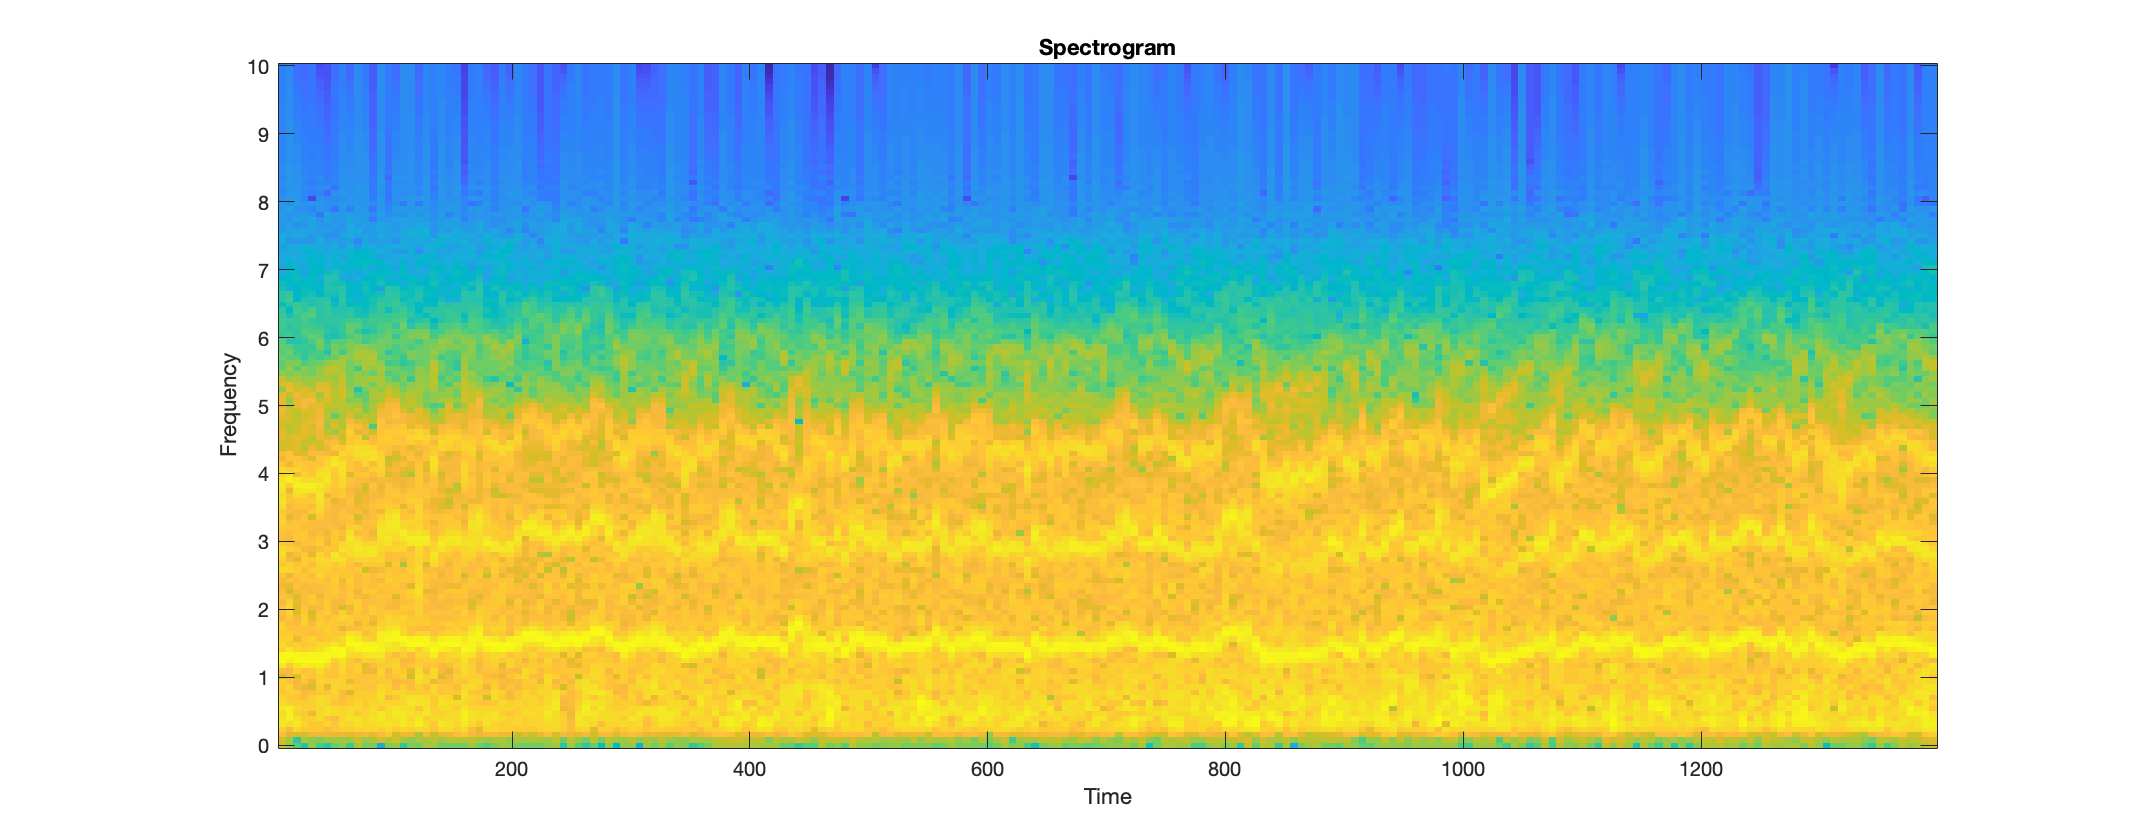
\includegraphics[width=85mm]{TL_sig3_spectrogram.png}
        \caption{Spectrogram of TL record.}
    \end{minipage}\hfill
\end{figure}

\noindent
Calculations of sample entropy of $3^{rd}$ signal from four selected recrods:
\begin{itemize}
    \item PE: $se = 1.58045$
    \item PL: $se = 1.21496$
    \item TE: $se = 1.99258$
    \item TL: $se = 1.64465$
\end{itemize}
Calculations of sample entropy of $2^{rd}$ signal from from four selected recrods:
\begin{itemize}
    \item PE: $se = 1.02238$
    \item PL: $se = 0.84793$
    \item TE: $se = 1.35166$
    \item TL: $se = 0.97777$
\end{itemize}
\noindent
For further analysis, we use the pre-calculated sample entropy, takem from \cite{bib:net}. 
Calculations of sample entropy may vary from previous, however the relationship between the results should be similar. 
\\
\noindent
On our results of calculated entropies, we do two-sample t-test. Function ttest2(X,Y) performs a t-test of the hypothesis that two
independent samples, in the vectors X and Y, come from distributions
with equal means, and returns the result of the test in H.  H=0
indicates that the null hypothesis ("means are equal") cannot be
rejected at the 5\% significance level.  H=1 indicates that the null
hypothesis can be rejected at the 5\% level.  The data are assumed to
come from normal distributions with unknown, but equal, variances.
\\
With t-test for all records ($3^{rd}$ signals) we get the result 
$$ H = 1 \ \text{and} \ P = 0.0139 $$
We also take a look at all records ($3^{rd}$ signal) and their sample entropies from website \cite{bib:fisio} and calculate the averages:
\begin{itemize}
    \item Mean sample entropy of PE records: $se = 0.935263$
    \item Mean sample entropy of PL records: $se = 0.912526$
    \item Mean sample entropy of TE records: $se = 0.999846$
    \item Mean sample entropy of TL records: $se = 0.949630$
    \item Mean sample entropy of all term records: $se = 0.977038$
    \item Mean sample entropy of all pre-term records: $se = 0.923895$
\end{itemize}
Finally, we do some visualizations of the sample entropy results, since the numbers do not really tell much.
\begin{figure}[ht!]
    \centering
    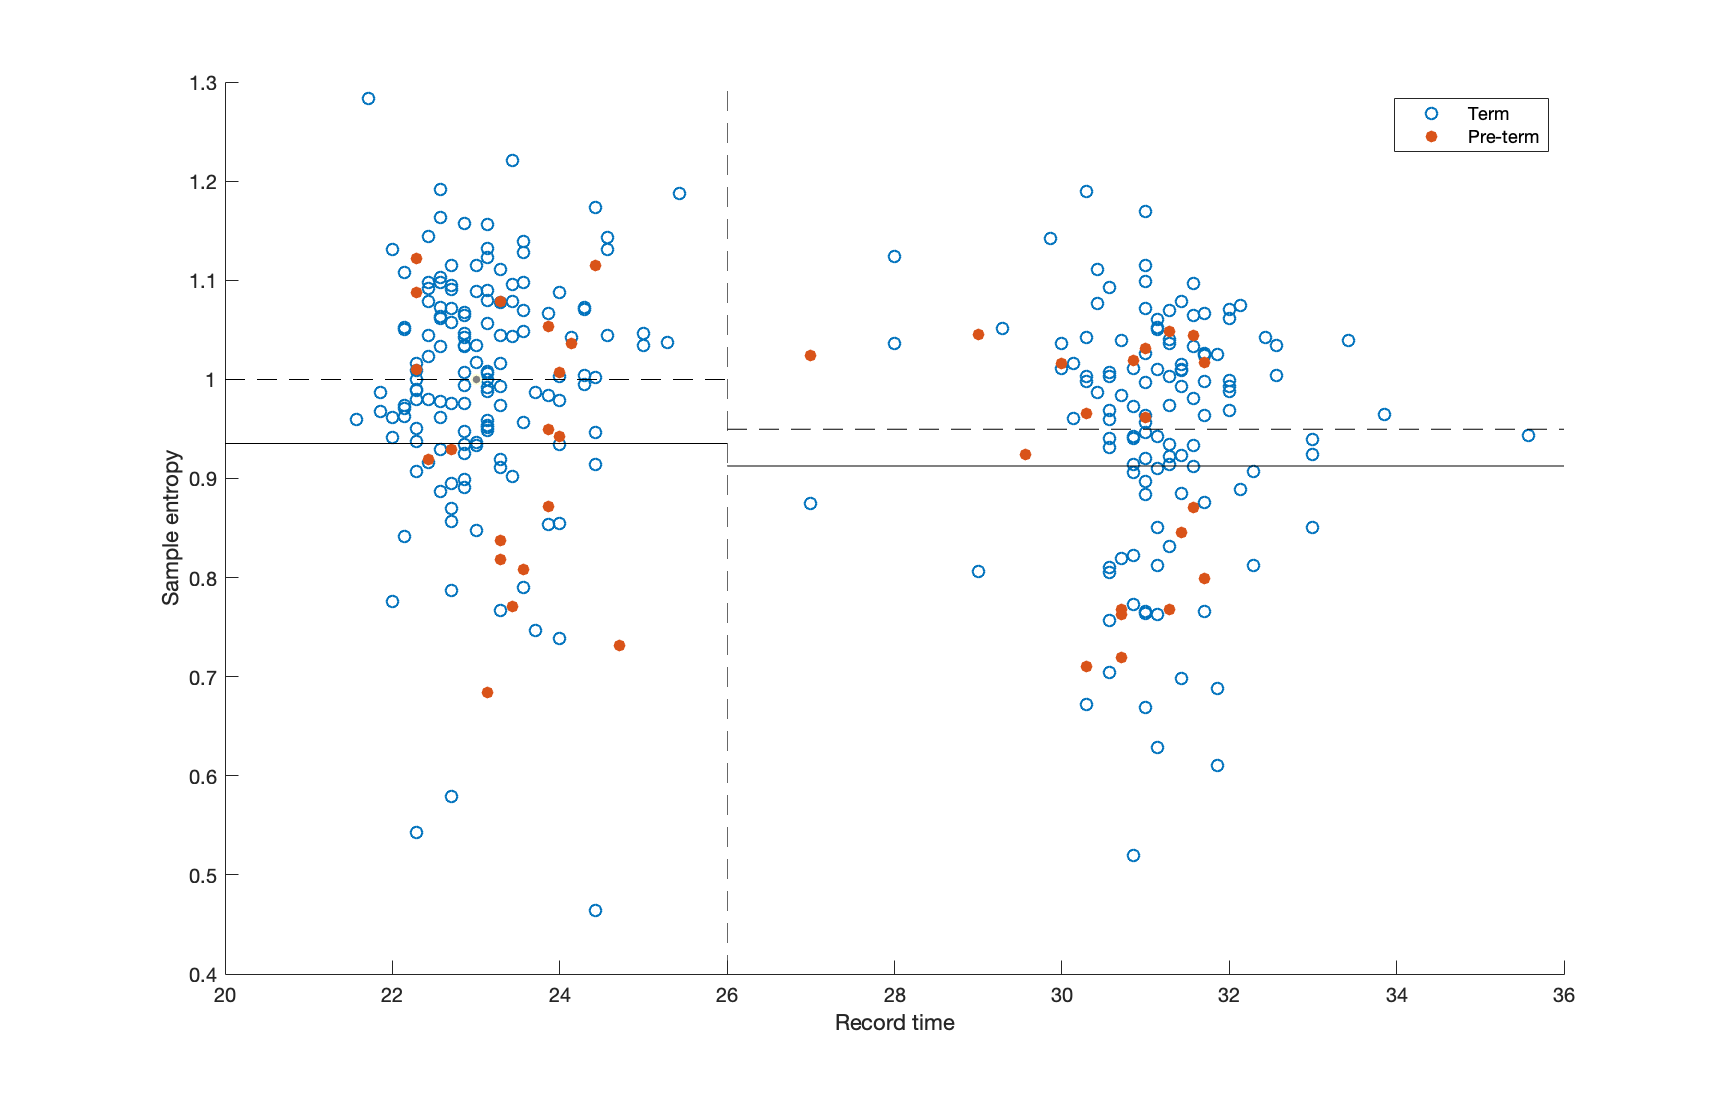
\includegraphics[width=150mm]{sample_averages.png}
    \caption{Sample entropy measurements as a fuction of time (record time in weeks). The dotted horizontal lines are the average sample entropy for term delivery records, the full horizontal lines are average sample entropy for pre-term records.}
\end{figure}

\begin{figure}[ht!]
    \centering
    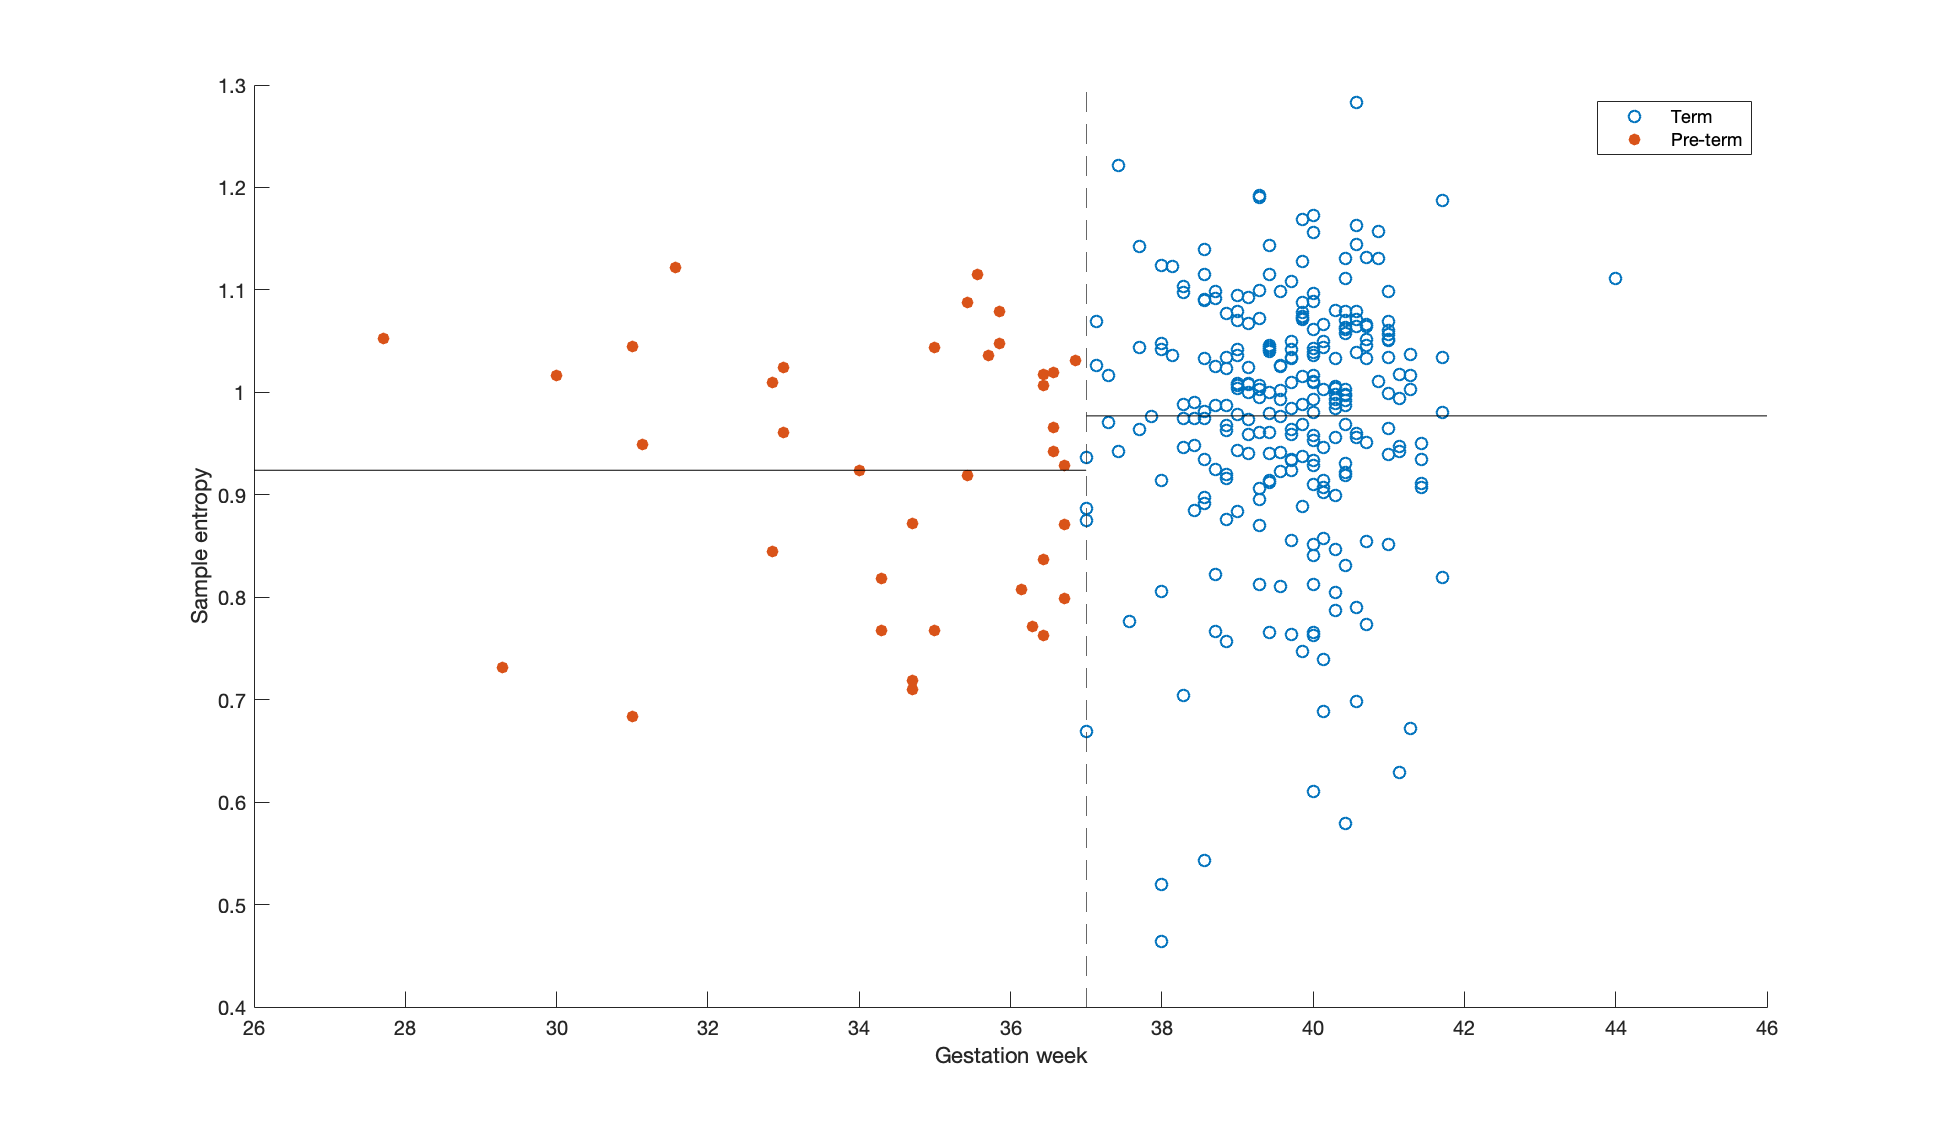
\includegraphics[width=150mm]{sample_entropy_gestation.png}
    \caption{Sample entropy measurements as a function of time (gestation week) with marked average entropy for term and pre-term.}
\end{figure}

\newpage
\section{Conclusion}
\ \
Predictability of early recorded signal is in general higher, and also predictability of record of pre-term labour, since the power spectrum already moved to lower frequencies which corresponds to higher predictability and lower sample entropy values.
\\
From the averages (and also from our four selected records) we can firstly see that sample entropy of term labour is higher than sample entropy of pre-term labour. 
It was expected, because when the labour is close, contractions are more regular and also stronger.
\\
Secondly, sample entropy of PE is higher than sample entropy of PL and the same goes for TE and TL (se(TE) > se(TL)).
\\
Lastly, sample entropy of TE is higher than sample entropy of PE and the same goes for TL and PL (se(TL) > se(PL)).
\\
\\
If we compare the sample entropy of $3^{rd}$ signals and $2^{rd}$ signals of records, we can quickly notice that sample entropy of the $2^{rd}$ signals is in general lower than sample entropy of the $3^{rd}$ signals,
so we can conclude that predictability of $2^{rd}$ signal is higher.

%%%%%%%%%%%%%%%%%%%%%%%%%%%%%%%%%%%%%%%%%%%

\begin{thebibliography}{99}

    \bibitem{bib:net}
    Gašper Fele-Žorž, Gorazd Kavšek, Živa Novak-Antolič and Franc Jager. \emph{A comparison of various linear and non-linear signal processing techniques to separate uterine EMG records of term and pre-term delivery groups}. Medical and Biological Engineering and Computing, 46(9):911-922 (2008).

    \bibitem{bib:fisio}
    Goldberger, A.~Amaral, L.~Glass, L.~Hausdorff, J.~Ivanov, P.~C.~Mark, Stanley, H. E. (2000). PhysioBank, PhysioToolkit, and PhysioNet: \emph{Components of a new research resource for complex physiologic signals}, Circulation [Online]. 101 (23), pp. e215–e220.

    \bibitem{bib:netcode}
    \emph{Sample entropy code}, [viewed 28.~12.~2020], available at \url{https://www.mathworks.com/matlabcentral/fileexchange/35784-sample-entropy}.

\end{thebibliography}

\end{document}